%%%%%%%%%%%%%%%%%%%%%%%%%%%%%%%%%%%%%%%%%%%%%%%%%%%%%%%%%%%%%%%%%%%%%%%%%%%%%%%%%%
\begin{frame}[fragile]\frametitle{}
\begin{center}
{\Large Decision Tree with Scikit-Learn}
\end{center}
\end{frame}

%%%%%%%%%%%%%%%%%%%%%%%%%%%%%%%%%%%%%%%%%%%%%%%%%%%%%%%%%%%%%%%%%%%%%%%%
\begin{frame}[fragile]\frametitle{Classification and Regression Trees (CART)}
\begin{lstlisting}
# Decision Tree Classifier
from sklearn import datasets
from sklearn import metrics
from sklearn.tree import DecisionTreeClassifier
# load the iris datasets
dataset = datasets.load_iris()
# fit a CART model to the data
model = DecisionTreeClassifier()
model.fit(dataset.data, dataset.target)
print(model)
# make predictions
expected = dataset.target
predicted = model.predict(dataset.data)
# summarize the fit of the model
print(metrics.classification_report(expected, predicted))
print(metrics.confusion_matrix(expected, predicted))
\end{lstlisting}

{\tiny (Ref: Machine Learning Algorithm Recipes in scikit-learn - Jason Brownlee)}

\end{frame}


% %%%%%%%%%%%%%%%%%%%%%%%%%%%%%%%%%%%%%%%%%%%%%%%%%%%%%%%%%%%%%%%%%%%%%%%%
% \begin{frame}[fragile]\frametitle{Decision Tree Sample Code}
% \begin{lstlisting}
% from sklearn import tree 

% #Assumed you have, X (predictor) and Y (target) for training data set and x_test(predictor) of test_dataset 

% model = tree.DecisionTreeClassifier(criterion='gini') 
% # model = tree.DecisionTreeRegressor() for regression 

% model.fit(X, y) 
% model.score(X, y) 

% predicted= model.predict(x_test) 
% \end{lstlisting}
% \end{frame}

% %%%%%%%%%%%%%%%%%%%%%%%%%%%%%%%%%%%%%%%%%%%%%%%%%%%%%%%%%%%%%%%%%%%%%%%%%%%%%%%%%%
% \begin{frame}[fragile]\frametitle{}
% \begin{center}
% {\Large Small Example: Vehicle Price Predictions}
% \end{center}
% \end{frame}


% %%%%%%%%%%%%%%%%%%%%%%%%%%%%%%%%%%%%%%%%%%%%%%%%%%%%%%%%%%%%%%%%%%%%%%%%
% \begin{frame}[fragile]\frametitle{Predicting Price of a Vehicle}
% \begin{lstlisting}
% import pandas as pd
% filename = 'vehicles_train.csv'
% url = 'https://raw.githubusercontent.com/justmarkham/DAT8/master/data/' + filename

% train = pd.read_csv(filename)
% \end{lstlisting}
% \begin{center}
% 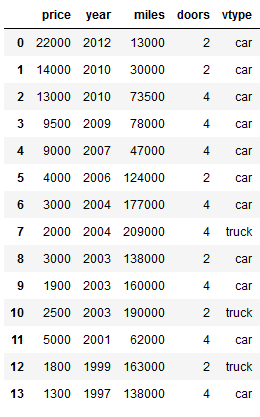
\includegraphics[width=0.4\linewidth]{car11}
% \end{center}
% \end{frame}


% %%%%%%%%%%%%%%%%%%%%%%%%%%%%%%%%%%%%%%%%%%%%%%%%%%%%%%%%%%%%%%%%%%%%%%%%
% \begin{frame}[fragile]\frametitle{Predicting Price of a Vehicle}
% \begin{lstlisting}
% # encode car as 0 and truck as 1
% train['vtype'] = train.vtype.map({'car':0, 'truck':1})

% # define X and y
% feature_cols = ['year', 'miles', 'doors', 'vtype']
% X = train[feature_cols]
% y = train.price

% from sklearn.tree import DecisionTreeRegressor

% treereg = DecisionTreeRegressor(random_state=1)

% # use leave-one-out cross-validation (LOOCV) to estimate the RMSE for this model
% from sklearn.model_selection import cross_val_score

% scores = cross_val_score(treereg, X, y, cv=14, scoring='r2')
% np.mean(np.sqrt(-scores))
% \end{lstlisting}
% \end{frame}


% %%%%%%%%%%%%%%%%%%%%%%%%%%%%%%%%%%%%%%%%%%%%%%%%%%%%%%%%%%%%%%%%%%%%%%%%
% \begin{frame}[fragile]\frametitle{Predicting Price of a Vehicle}
% \begin{center}
% 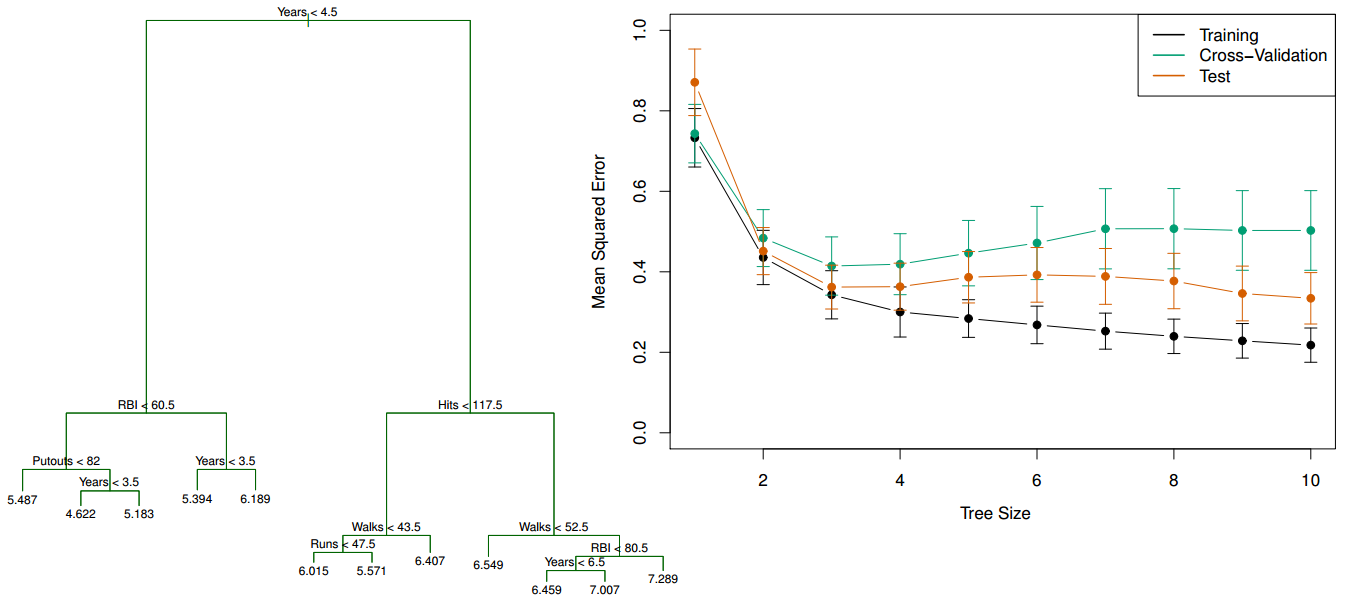
\includegraphics[width=\linewidth]{car2}
% \end{center}
% \end{frame}


% %%%%%%%%%%%%%%%%%%%%%%%%%%%%%%%%%%%%%%%%%%%%%%%%%%%%%%%%%%%%%%%%%%%%%%%%
% \begin{frame}[fragile]\frametitle{Tuning a regression tree}
% Let's try to reduce the RMSE by tuning the max\_depth parameter:
% \begin{lstlisting}
% # try different values one-by-one
% treereg = DecisionTreeRegressor(max_depth=1, random_state=1)
% scores = cross_val_score(treereg, X, y, cv=14, scoring='mean_squared_error')
% np.mean(np.sqrt(-scores))

% 3757.936507936508
% # plot max_depth (x-axis) versus RMSE (y-axis)
% plt.plot(max_depth_range, RMSE_scores)
% plt.xlabel('max_depth')
% plt.ylabel('RMSE (lower is better)')
% \end{lstlisting}
% \begin{center}
% 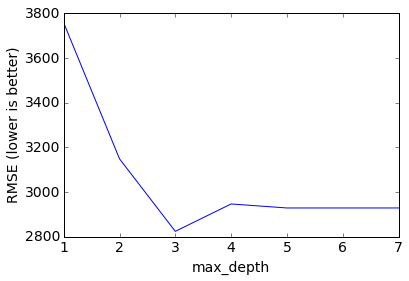
\includegraphics[width=0.4\linewidth]{car3}
% \end{center}
% \end{frame}

% %%%%%%%%%%%%%%%%%%%%%%%%%%%%%%%%%%%%%%%%%%%%%%%%%%%%%%%%%%%%%%%%%%%%%%%%
% \begin{frame}[fragile]\frametitle{Tuning a regression tree}
% max\_depth=3 was best, so fit a tree using that parameter
% \begin{lstlisting}
% # max_depth=3 was best, so fit a tree using that parameter
% treereg = DecisionTreeRegressor(max_depth=3, random_state=1)
% treereg.fit(X, y)
% \end{lstlisting}
% ``Gini importance'' of each feature: the (normalized) total reduction of error brought by that feature
% \begin{lstlisting}
% pd.DataFrame({'feature':feature_cols, 'importance':treereg.feature_importances_})
% \end{lstlisting}
% \begin{center}
% 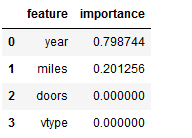
\includegraphics[width=0.3\linewidth]{car4}
% \end{center}
% \end{frame}

% %%%%%%%%%%%%%%%%%%%%%%%%%%%%%%%%%%%%%%%%%%%%%%%%%%%%%%%%%%%%%%%%%%%%%%%%
% \begin{frame}[fragile]\frametitle{Creating a tree diagram}
% \begin{lstlisting}
% from sklearn.tree import export_graphviz

% export_graphviz(treereg, out_file='tree_vehicles.dot', feature_names=feature_cols)
% \end{lstlisting}
% \begin{center}
% 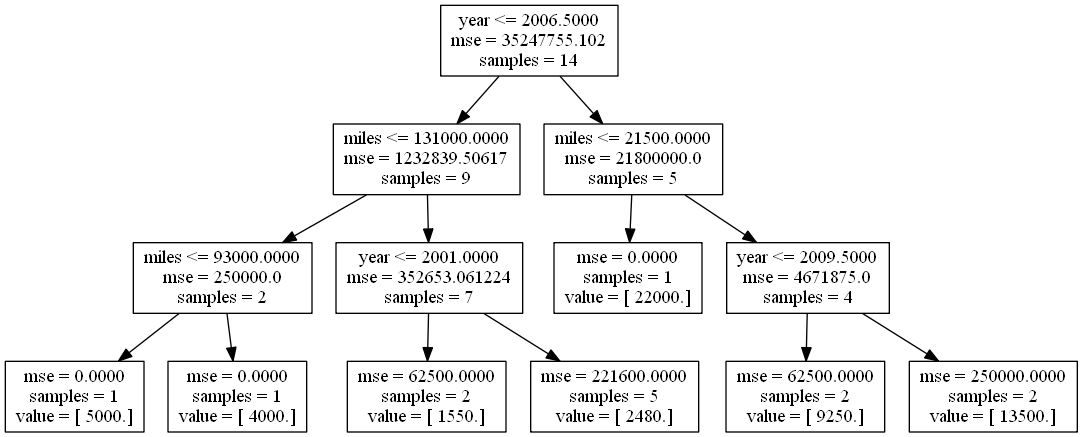
\includegraphics[width=0.95\linewidth]{car5}
% \end{center}
% \end{frame}

% %%%%%%%%%%%%%%%%%%%%%%%%%%%%%%%%%%%%%%%%%%%%%%%%%%%%%%%%%%%%%%%%%%%%%%%%
% \begin{frame}[fragile]\frametitle{Making predictions for the testing data}
% \begin{lstlisting}
% # use fitted model to make predictions on testing data
% X_test = test[feature_cols]
% y_test = test.price
% y_pred = treereg.predict(X_test)

% # calculate RMSE
% np.sqrt(metrics.mean_squared_error(y_test, y_pred))

% # calculate RMSE for your own tree!
% y_test = [3000, 6000, 12000]
% y_pred = [0, 0, 0]
% from sklearn import metrics
% np.sqrt(metrics.mean_squared_error(y_test, y_pred))
% \end{lstlisting}

% \end{frame}

% %%%%%%%%%%%%%%%%%%%%%%%%%%%%%%%%%%%%%%%%%%%%%%%%%%%%%%%%%%%%%%%%%%%%%%%%%%%%%%%%%%
% \begin{frame}[fragile]\frametitle{}
% \begin{center}
% {\Large Test case: Car Valuation}
% \end{center}
% \end{frame}

% %%%%%%%%%%%%%%%%%%%%%%%%%%%%%%%%%%%%%%%%%%%%%%%%%%%%%%%%%%%%%%%%%%%%%%%%
% \begin{frame}[fragile]\frametitle{Decision Trees}
% \begin{itemize}
% \item Since decision trees are good algorithms for discovering the structure hidden behind data, we'll use and model the car evaluation data set.
% \item Source: http://archive.ics.uci.edu/ml/machine-learning-databases/car/
% \item CAR car acceptability:
		% \begin{itemize}
		% \item  buying buying price
		% \item  maint price of the maintenance
		% \item  doors number of doors
		% \item    persons capacity in terms of persons to carry
		% \item   lug\_boot the size of luggage boot
		% \item  safety estimated safety of the car
		% \end{itemize}
% \end{itemize}
% \end{frame}

% %%%%%%%%%%%%%%%%%%%%%%%%%%%%%%%%%%%%%%%%%%%%%%%%%%%%%%%%%%%%%%%%%%%%%%%%
% \begin{frame}[fragile]\frametitle{Decision Trees: Dataset}
% \begin{itemize}
% \item Number of Attributes: 6
% \item Missing Attribute Values: none
% \item Values:
		% \begin{itemize}
		% \item  buying: 	v-high, high, med, low
		% \item  maint: 	v-high, high, med, low
		% \item  doors: 	2, 3, 4, 5-more
		% \item  persons: 	2, 4, more
		% \item  lug\_boot: 	small, med, big
		% \item  safety:	low, med, high
		% \end{itemize}
% \item Number of Instances: 1728 (Instances completely cover the attribute space.)
% \end{itemize}
% \end{frame}

% %%%%%%%%%%%%%%%%%%%%%%%%%%%%%%%%%%%%%%%%%%%%%%%%%%%%%%%%%%%%%%%%%%%%%%%%
% \begin{frame}[fragile]\frametitle{Imports}
% \begin{lstlisting}
% import numpy as np
% import pandas as pd
% import matplotlib.pyplot as plt
% from sklearn.preprocessing import LabelEncoder, OneHotEncoder
% from sklearn import tree
% import pydot

% from io import StringIO
% import os
% \end{lstlisting}
% \end{frame}



% %%%%%%%%%%%%%%%%%%%%%%%%%%%%%%%%%%%%%%%%%%%%%%%%%%%%%%%%%%%%%%%%%%%%%%%%
% \begin{frame}[fragile]\frametitle{Get Data}
% \begin{lstlisting}
% # Load data set
% data = np.genfromtxt(os.path.join('data', 'car.data'), delimiter=',', dtype="U")
% data_inputs = data[:, :-1]
% data_outputs = data[:, -1]
% \end{lstlisting}
% \end{frame}

% %%%%%%%%%%%%%%%%%%%%%%%%%%%%%%%%%%%%%%%%%%%%%%%%%%%%%%%%%%%%%%%%%%%%%%%%
% \begin{frame}[fragile]\frametitle{Define the features and preprocess the car evaluation data set}
% \begin{lstlisting}
% # The integer values for features will take
% # a range from 0 to n-1 in the lists of possible values:
% input_labels = [
    % ["buying", ["vhigh", "high", "med", "low"]],
    % ["maint", ["vhigh", "high", "med", "low"]],
    % ["doors", ["2", "3", "4", "5more"]],  # Here indexes are not real values
    % ["persons", ["2", "4", "more"]],
    % ["lug_boot", ["small", "med", "big"]],
    % ["safety", ["low", "med", "high"]],
% ]

% class_names = ["unacc", "acc", "good", "vgood"]
% \end{lstlisting}
% \end{frame}

% %%%%%%%%%%%%%%%%%%%%%%%%%%%%%%%%%%%%%%%%%%%%%%%%%%%%%%%%%%%%%%%%%%%%%%%%
% \begin{frame}[fragile]\frametitle{Encode Categorical Variables}
% \begin{lstlisting}
% def str_data_to_one_hot(data, input_labels):
    % """Convert each feature's string to a flattened one-hot array. """
    % X_int = LabelEncoder().fit_transform(data.ravel()).reshape(*data.shape)
    % X_bin = OneHotEncoder().fit_transform(X_int).toarray()
    
    % feature_names = []
    % for a in input_labels:
        % key = a[0]
        % for b in a[1]:
            % value = b
            % feature_names.append("{}_is_{}".format(key, value))

    % return X_bin, feature_names
% \end{lstlisting}
% \end{frame}

% %%%%%%%%%%%%%%%%%%%%%%%%%%%%%%%%%%%%%%%%%%%%%%%%%%%%%%%%%%%%%%%%%%%%%%%%
% \begin{frame}[fragile]\frametitle{Integer Variables}
% \begin{lstlisting}
% def str_data_to_linear(data, input_labels):
    % """Convert each feature's string to an integer index"""
    % X_lin = np.array([[
        % input_labels[a][1].index(j) for a, j in enumerate(i)
    % ] for i in data])
    
    % # Integer feature indexes will range
    % # from 0 to n-1 from indexes in the label list:
    % feature_names = [i[0] + "_index" for i in input_labels]
    
    % return X_lin, feature_names
% \end{lstlisting}
% \end{frame}


% %%%%%%%%%%%%%%%%%%%%%%%%%%%%%%%%%%%%%%%%%%%%%%%%%%%%%%%%%%%%%%%%%%%%%%%%
% \begin{frame}[fragile]\frametitle{Encode Input}
% \begin{lstlisting}
% # Take both one-hot and linear versions of input features: 
% X_one_hot, feature_names_one_hot = str_data_to_one_hot(data_inputs, input_labels)
% X_linear_int, feature_names_linear_int = str_data_to_linear(data_inputs, input_labels)

% # Put that together:
% X = np.concatenate([X_one_hot, X_linear_int], axis=-1)
% feature_names = feature_names_one_hot + feature_names_linear_int
% \end{lstlisting}
% \end{frame}


% %%%%%%%%%%%%%%%%%%%%%%%%%%%%%%%%%%%%%%%%%%%%%%%%%%%%%%%%%%%%%%%%%%%%%%%%
% \begin{frame}[fragile]\frametitle{Encode Output}
% \begin{lstlisting}
% # Outputs use indexes, this is not one-hot:
% integer_y = np.array([class_names.index(i) for i in data_outputs])

% print("Data set's shape,")
% print("X.shape, integer_y.shape, len(feature_names), len(class_names):")
% print(X.shape, integer_y.shape, len(feature_names), len(class_names))
% \end{lstlisting}
% \end{frame}

% %%%%%%%%%%%%%%%%%%%%%%%%%%%%%%%%%%%%%%%%%%%%%%%%%%%%%%%%%%%%%%%%%%%%%%%%
% \begin{frame}[fragile]\frametitle{Train a simple decision tree to fit the data set}
% \begin{lstlisting}
% max_depth = 6
% clf = tree.DecisionTreeClassifier(max_depth=max_depth)
% clf = clf.fit(X, integer_y)

% print("Decision tree trained!")
% accuracy = clf.score(X, integer_y)
% print("Errors:", 100 - accuracy * 100, "%")
% print("Accuracy:", accuracy * 100, "%")
% \end{lstlisting}
% \end{frame}

% %%%%%%%%%%%%%%%%%%%%%%%%%%%%%%%%%%%%%%%%%%%%%%%%%%%%%%%%%%%%%%%%%%%%%%%%
% \begin{frame}[fragile]\frametitle{Plot and save the tree}
% \begin{lstlisting}
% def plot_first_tree(clf, class_names, tree_name):
    % graph_save_path = os.path.join(
        % "exported_sklearn_trees", 
        % "{}".format(tree_name)
    % )

    % tree.export_graphviz(clf, out_file="{}.dot".format(graph_save_path))
    % dotfile = StringIO()
    % tree.export_graphviz(
        % clf, out_file=dotfile,
        % feature_names=feature_names, class_names=class_names,
        % filled=True, rotate=True
    % )
    % pydot.graph_from_dot_data(dotfile.getvalue())[0].write_png("{}.png".format(graph_save_path))

% # Plot our simple tree:
% plot_first_tree(clf, class_names, tree_name="simple_tree")
% \end{lstlisting}
% \end{frame}

% %%%%%%%%%%%%%%%%%%%%%%%%%%%%%%%%%%%%%%%%%%%%%%%%%%%%%%%%%%%%%%%%%%%%%%%%
% \begin{frame}[fragile]\frametitle{Plot}
% \begin{center}
% 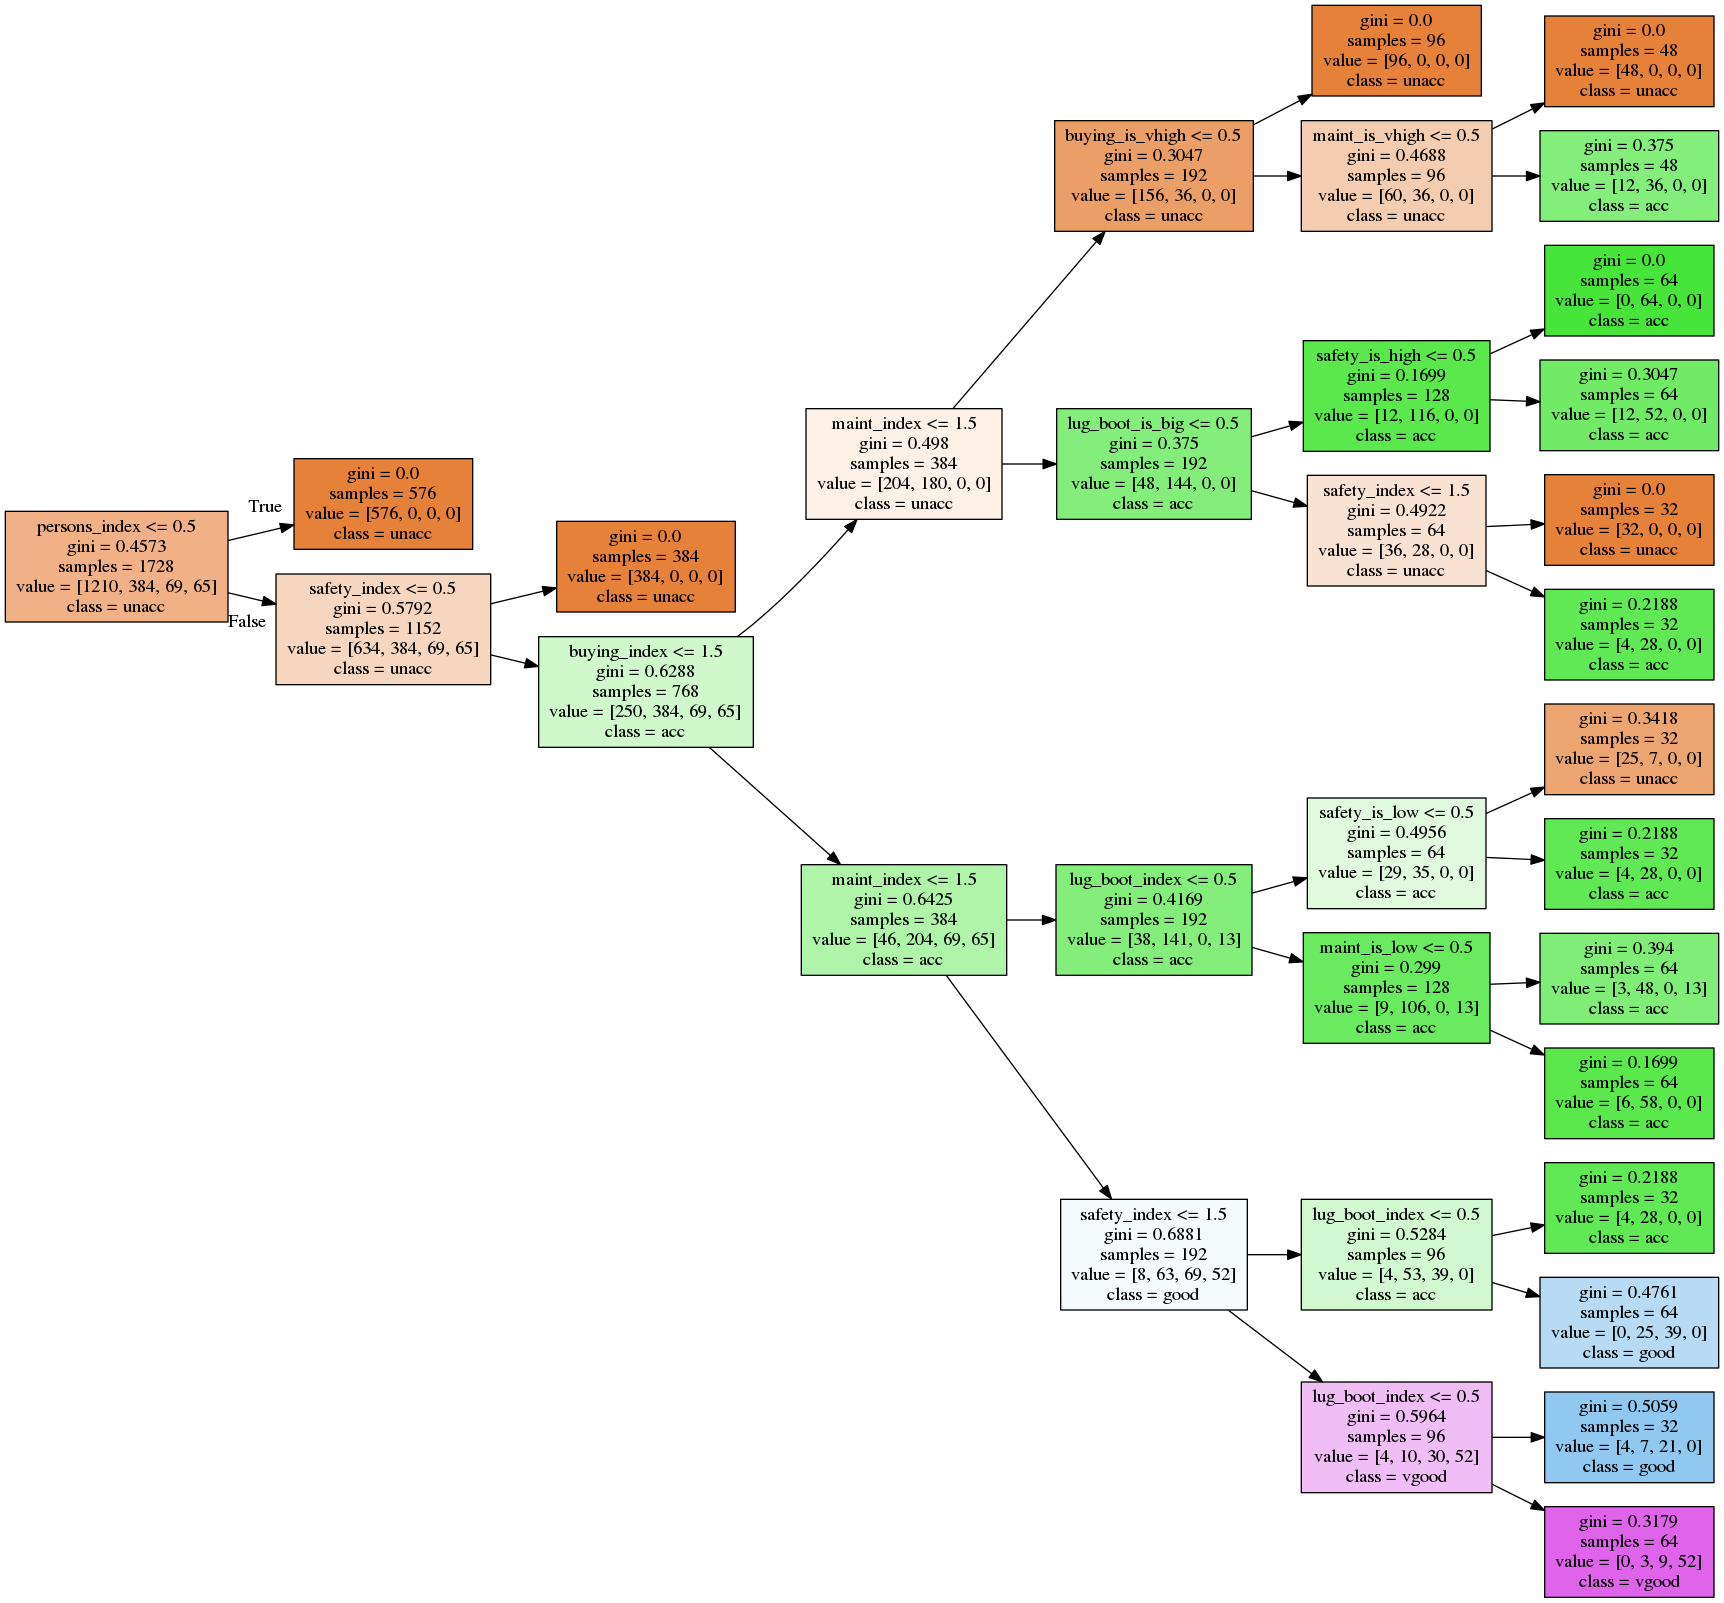
\includegraphics[width=0.6\linewidth]{rfp1}
% \end{center}
% \end{frame}

% %%%%%%%%%%%%%%%%%%%%%%%%%%%%%%%%%%%%%%%%%%%%%%%%%%%%%%%%%%%%%%%%%%%%%%%%
% \begin{frame}[fragile]\frametitle{Plot the importance of each input features}
% \begin{lstlisting}
% def feature_importance_chart(clf, classifier_name, feature_names):
    % sorted_feature_importances, sorted_feature_names = (
        % zip(*sorted(zip(clf.feature_importances_, feature_names)))
    % )
    % plt.figure(figsize=(16, 9))
    % plt.barh(range(len(sorted_feature_importances)), sorted_feature_importances)
    % plt.yticks(
        % range(len(sorted_feature_importances)),
        % ["{}: {:.3}".format(a, b) for a, b in zip(sorted_feature_names, sorted_feature_importances)]
    % )
    % plt.title("The Gini feature importance for the {} \n"
              % "(total decrease in node impurity, weighted by the "
              % "probability of reaching that node)".format(classifier_name))
    % plt.show()

% feature_importance_chart(clf, "simple tree", feature_names)
% \end{lstlisting}
% \end{frame}

% %%%%%%%%%%%%%%%%%%%%%%%%%%%%%%%%%%%%%%%%%%%%%%%%%%%%%%%%%%%%%%%%%%%%%%%%
% \begin{frame}[fragile]\frametitle{Plot}
% \begin{center}
% 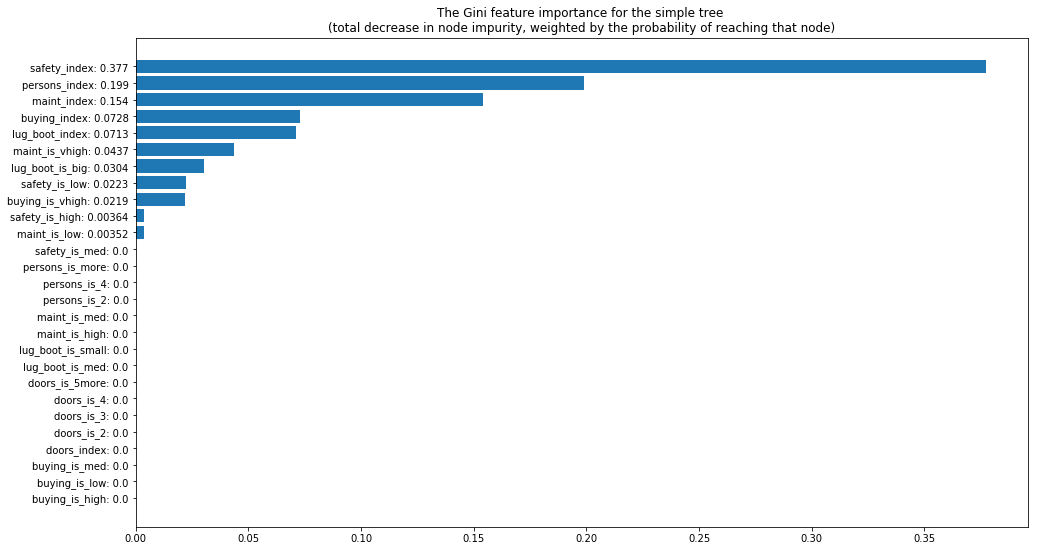
\includegraphics[width=\linewidth]{rfp2}
% \end{center}
% \end{frame}


% %%%%%%%%%%%%%%%%%%%%%%%%%%%%%%%%%%%%%%%%%%%%%%%%%%%%%%%%%%%%%%%%%%%%%%%%
% \begin{frame}[fragile]\frametitle{A fully perfect (complex) tree}
% \begin{lstlisting}
% max_depth = None  # Full depth
% clf = tree.DecisionTreeClassifier(max_depth=max_depth)
% clf = clf.fit(X, integer_y)

% print("Decision tree trained!")
% accuracy = clf.score(X, integer_y)
% print("Errors:", 100 - accuracy * 100, "%")
% print("Accuracy:", accuracy * 100, "%")

% plot_first_tree(clf, class_names, tree_name="complex_tree")
% \end{lstlisting}
% \end{frame}


% %%%%%%%%%%%%%%%%%%%%%%%%%%%%%%%%%%%%%%%%%%%%%%%%%%%%%%%%%%%%%%%%%%%%%%%%
% \begin{frame}[fragile]\frametitle{Plot}
% \begin{center}
% 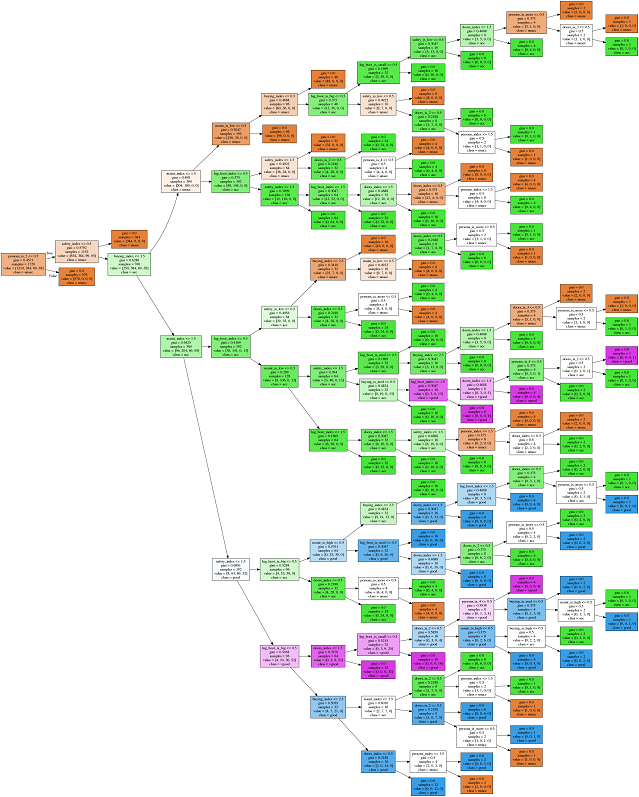
\includegraphics[width=0.5\linewidth]{rfp3}
% \end{center}
% \end{frame}

% %%%%%%%%%%%%%%%%%%%%%%%%%%%%%%%%%%%%%%%%%%%%%%%%%%%%%%%%%%%%%%%%%%%%%%%%
% \begin{frame}[fragile]\frametitle{Full feature importance}
% \begin{center}
% 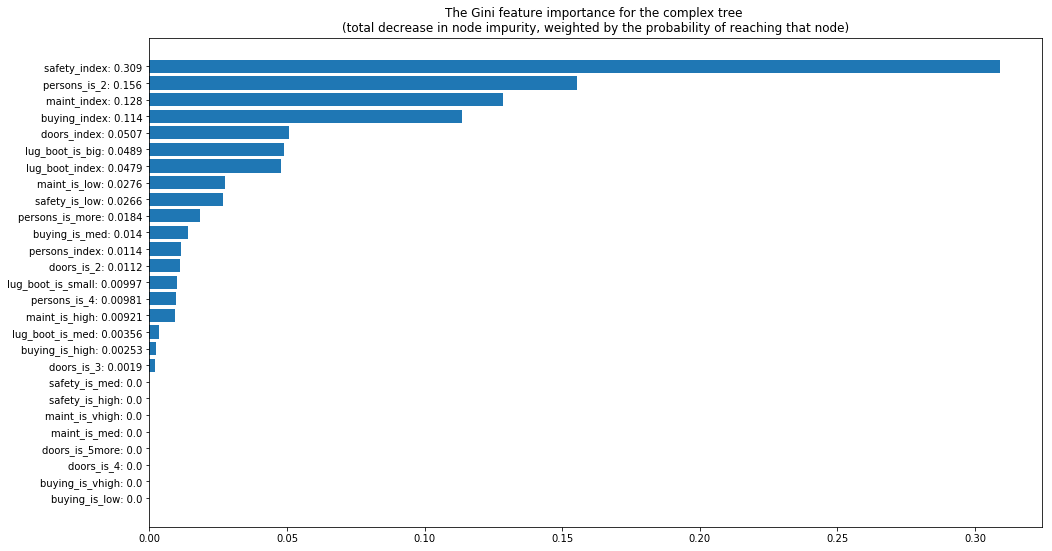
\includegraphics[width=\linewidth]{rfp4}
% \end{center}
% \end{frame}

% %%%%%%%%%%%%%%%%%%%%%%%%%%%%%%%%%%%%%%%%%%%%%%%%%%%
% \begin{frame}[fragile] \frametitle{Decision Tree (Recap)}
% \begin{itemize}
% \item able to interpret the important variables in a model
% \item handles missing values well in both training and testing data
% \item reasonably fast to train
% \item does not depend on the scale of the predictor variables
% \item can handle multiclass problems directly
% \item works natively with categorical variables
% \item easily modified to be robust to outliers (just replace MSE with MAD
% for evaluating splits; means with medians for predictions in terminal nodes)
% \item very fast to classify new points
% \item robust to tuning parameters (the stopping criteria), \textit{for a given set of data}
% \end{itemize}
% \end{frame}
